
\documentclass[a4]{beamer}
\usepackage{amssymb}
\usepackage{graphicx}
\usepackage{subfigure}
\usepackage{newlfont}
\usepackage{amsmath,amsthm,amsfonts}
%\usepackage{beamerthemesplit}
\usepackage{pgf,pgfarrows,pgfnodes,pgfautomata,pgfheaps,pgfshade}
\usepackage{mathptmx} % Font Family
\usepackage{helvet} % Font Family
\usepackage{color}
\mode<presentation> {
\usetheme{Default} % was Frankfurt
\useinnertheme{rounded}
\useoutertheme{infolines}
\usefonttheme{serif}
%\usecolortheme{wolverine}
% \usecolortheme{rose}
\usefonttheme{structurebold}
}
\setbeamercovered{dynamic}
\title[MA4413]{Statistics for Computing \\ {\normalsize MA4413 Lecture 10B}}
\author[Kevin O'Brien]{Kevin O'Brien \\ {\scriptsize Kevin.obrien@ul.ie}}
\date{Autumn Semester 2013}
\institute[Maths \& Stats]{Dept. of Mathematics \& Statistics, \\ University \textit{of} Limerick}

\renewcommand{\arraystretch}{1.5}
%----------------------------------------------------------------------------------------------------------%
\begin{document}




%-------------------------------------------------%
[fragile]
\noindent \textbf{Graphical Procedures for assessing Normality}

\begin{itemize}
\item The normal probability (Q-Q) plot is a very useful tool for determining whether or not a data set is normally distributed.
\item Interpretation is simple. If the points follow the trendline (provided by the second line of \texttt{R} code \texttt{qqline}), then the data set can be assumed to be normally distributed.
\item One should expect minor deviations. Numerous major deviations would lead the analyst to conclude that the data set is not normally distributed.
\item The Q-Q plot is best used in conjunction with a formal procedure such as the Shapiro-Wilk test.
\end{itemize}

\begin{verbatim}
>qqnorm(CWdiff)
>qqline(CWdiff)
\end{verbatim}



%-------------------------------------------------%


\noindent \textbf{Graphical Procedures for Assessing Normality}

\begin{center}
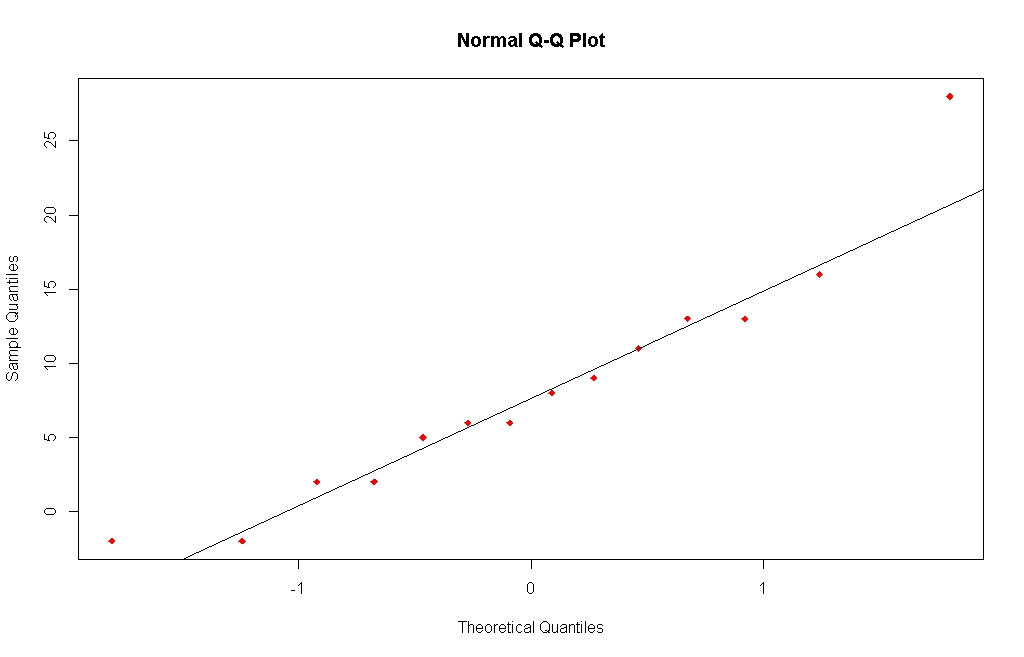
\includegraphics[scale=0.32]{10AQQplot}
\end{center}


\end{document}
